\subsection{Resumen}

Para imágenes suficientemente grandes, donde la cache no es suficiente, los filtros en asm con simd son muuucho mas rápido que los hechos en c: Analizaremos a partir de que tamaño de imagen la cache no es suficiente. Luego veremos como se comportan los filtros

\\
\subsection{Resultados:}\\

Nuestra hipotesis se basa en que asembler consigue un mejor uso de la cache, y le atribuimos a eso su velocidad, para comprobar eso observaremos los miss/hit de los diferentes filtros. Usaramos imagenes chicas y muy pesadas , el objetivo es ver si cuando la imagen es mas grande que la cache, los miss/hit de la misma cambian mucho o no en comparacion a los de las imagenes chicas. En este caso haremos tests en una computadora que tiene una cache de 6mb, por lo que usaremos imagenes que tienen un peso superior al de ese valor. 

\\
Con esto esperamos corroborar que los filtros implementados en asembler con simd tienen mas hit que los de c en situaciones que incluyen tanto a procesar una imagen mas grande que la cache como con una mas chica, y por ende son mucho mas rapidos que los de c. Queremos ver asi, si implementar codigo directamente en Asm resulta en un mejor uso de la cache, y entonces concluir que esto es una de las razones de lo rapido que son los filtros en Asm con respecto a los de c. A medida que relizamos los experimentos iremos incrementado el tamaño de la imagen para ver si la relacion Miss/Hit de ambos filtros va variando o no. Con cada tamaño de imagen ademas variaremos los parametros del filtro. 

\\
Los siguientes experimentos los realizamos sobre el filtro blur, ya que como este es mas complicado y tiene mas ciclos conideramos que le exige mas al predictor de saltos, ademas al no ser lineal el contenido de la cache cambiara con mas frecuencia, y asi las diferencias en el uso de cache, si es que las hay, seran mas pronunciadas. Este filtro ademas recibe parametros, si bien cambiar sigma no altera el uso de la cache (pues solo afecta cuentas), cambiar el radio produciria que mientras este aumente, se utilice una parte de la imagen completamente diferente e inesperada, por eso decidimos ahcer las pruebas con este filtro.

\\
Para ver los el uso de la cache utilizaremos el programa valgrind y relizaremos cada experimento viarias veces para obtener un promedio sacando outliers. Fijamos como 30 el radio maximo ya que si lo incrementabamos mas, porque el  valgrind demoraba demasiado en emular el comportamiento de la cache. A continuacion mostraremos algunos resultados obtenidos con las diferentes imagenes, mostrando su peso y porcentaje de miss. \\

2560x1080 8,3mb \\

Asm \\
	Radio 10   instruccion miss   0.0$\%$  data cache miss  4.1$\%$ miss jumps   4.5$\%$ \\
	Radio 20   instruccion miss   0.0$\%$  data cache miss  3.9$\%$ miss jumps   2.3$\%$ \\	
	Radio 30   instruccion miss   0.0$\%$  data cache miss  2.6$\%$ miss jumps   1.5$\%$ \\

C: \\
	Radio 10  instruccion miss  0.0$\%$  data cache miss 0.2$\%$ miss jumps  3.9 $\%$  \\
	Radio 20  instruccion miss  0.0$\%$  data cache miss 0.2$\%$ miss jumps   1.9 $\%$  \\
	Radio 30  instruccion miss  0.0$\%$  data cache miss 0.2$\%$ miss jumps   1.2$\%$  \\ 

1920x1080 6,2mb \\

Asm \\
	Radio 10   instruccion miss   0.0$\%$  data cache miss  0.5$\%$ miss jumps   4.5$\%$ \\
	Radio 20   instruccion miss   0.0$\%$  data cache miss  4.5$\%$ miss jumps   2.4$\%$ \\	
	Radio 30   instruccion miss   0.0$\%$  data cache miss  4.6$\%$ miss jumps   1.6$\%$ \\

C: \\
	Radio 10  instruccion miss  0.0$\%$  data cache miss 0.0$\%$ miss jumps  4.4 $\%$  \\
	Radio 20  instruccion miss  0.0$\%$  data cache miss 0.2$\%$ miss jumps   2.3 $\%$  \\
	Radio 30  instruccion miss  0.0$\%$  data cache miss 0.2$\%$ miss jumps   1.5$\%$  \\ 

1280x720 2,8mb \\

Asm \\
	Radio 10 instruccion miss   0.0$\%$  data cache miss  0.5$\%$ miss jumps   4.5$\%$ \\
	Radio 20 instruccion miss   0.0$\%$  data cache miss  4.5$\%$ miss jumps   2.4$\%$ \\	
	Radio 30 instruccion miss   0.0$\%$  data cache miss  4.6$\%$ miss jumps   1.6$\%$ \\

C: \\
	Radio 10 instruccion miss  0.0$\%$  data cache miss 0.0$\%$ miss jumps  4.4 $\%$  \\
	Radio 20 instruccion miss  0.0$\%$  data cache miss 0.2$\%$ miss jumps   2.3 $\%$  \\
	Radio 30 instruccion miss  0.0$\%$  data cache miss 0.2$\%$ miss jumps   1.5$\%$  \\ 

1024x600 1,8mb \\

Asm:\\ 
	Radio 10 600  	instruccion miss 0.0$\%$  data cache miss  4.1 $\%$ miss jumps  4.5$\%$  \\
	Radio 20 600  instruccion miss 0.0$\%$  data cache miss  4.0$\%$ miss jumps 2.4$\%$     \\
	Radio 30 600  	instruccion miss 0.0$\%$  data cache miss  3.9$\%$ miss jumps   1.6$\%$   \\

C: \\
	Radio 10 600  	instruccion miss  0.0$\%$ data cache miss 0.2 $\%$ miss jumps  4.4$\%$ \\
	Radio 20 600  	instruccion miss  0.0$\%$ data cache miss 0.1$\%$ miss jumps 2.2$\%$ \\
	Radio 30 600  	instruccion miss  0.0$\%$ data cache miss 0.1$\%$ miss jumps  1.5$\%$ \\

320x480 600k \\

Asm: \\
	Radio 10 480  	instruccion miss 0.0$\%$  data cache miss  0.2 $\%$ miss jumps  4.5$\%$	\\
	Radio 20 480  instruccion miss 0.0$\%$  data cache miss  0.3$\%$ miss jumps 2.4$\%$	\\
	Radio 30 480  	instruccion miss 0.0$\%$  data cache miss  1.9$\%$ miss jumps   1.6$\%$	\\

C:\\
	Radio 10 480  	instruccion miss  0.0$\%$ data cache miss 0.0 $\%$ miss jumps  4.4$\%$ \\
	Radio 20 480  	instruccion miss  0.0$\%$ data cache miss 0.0$\%$ miss jumps 2.3$\%$ \\
	Radio 30 480  	instruccion miss  0.0$\%$ data cache miss 0.0$\%$ miss jumps  1.5$\%$ \\

\subsection{Graficos:} \\


\begin{figure}[H]
\begin{center}
  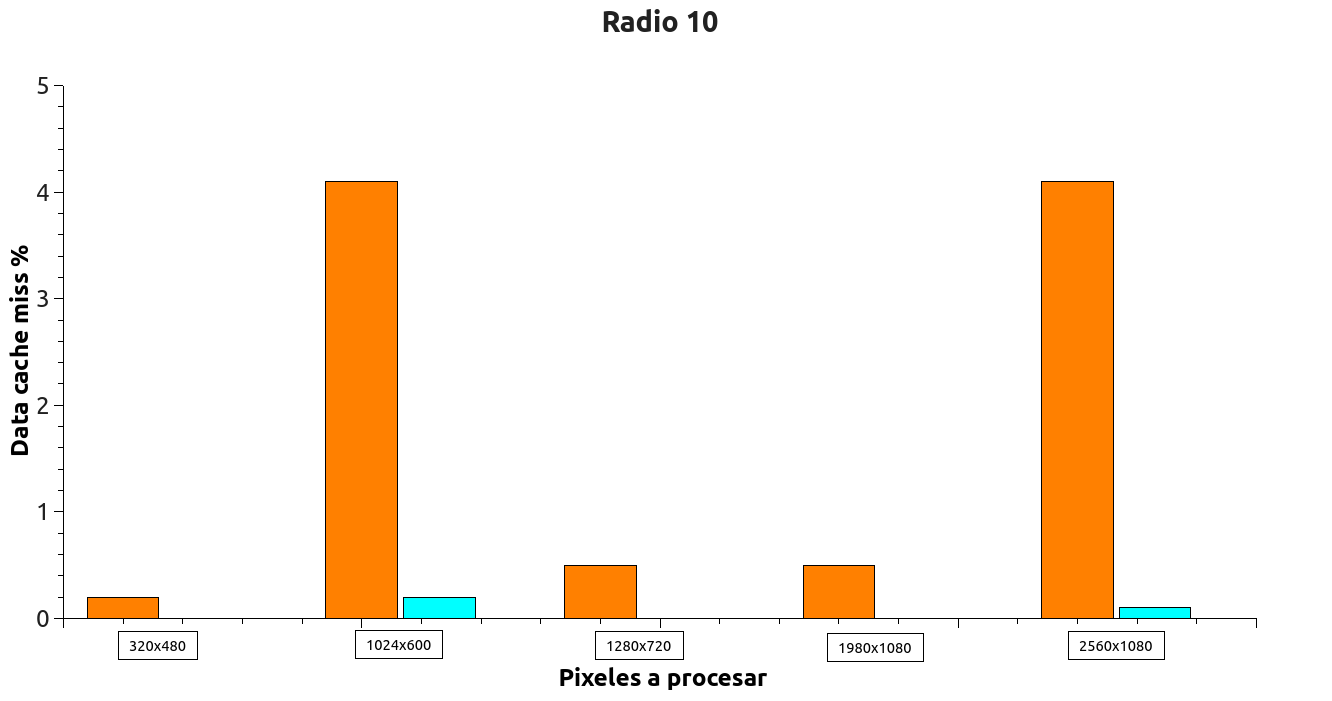
\includegraphics[width=\linewidth]{cache/Radio 10.png}
\end{center}
\end{figure}

\begin{figure}[H]
\begin{center}
  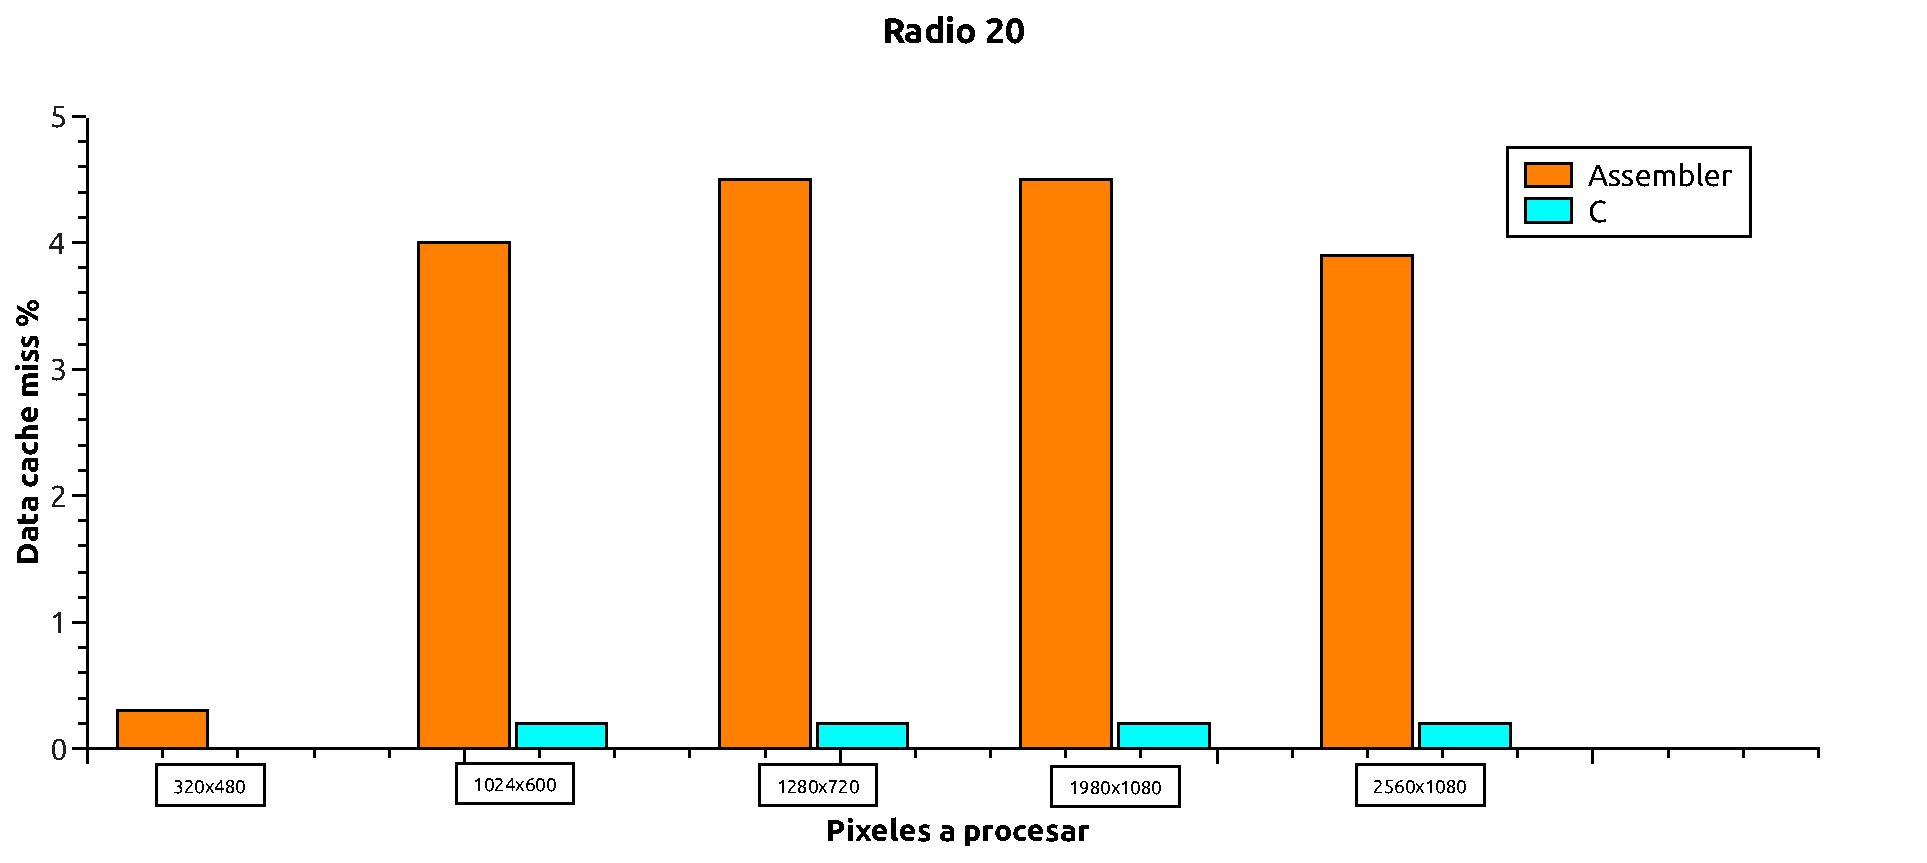
\includegraphics[width=\linewidth]{cache/Radio 20.pdf}
\end{center}
\end{figure}

\begin{figure}[H]
\begin{center}
  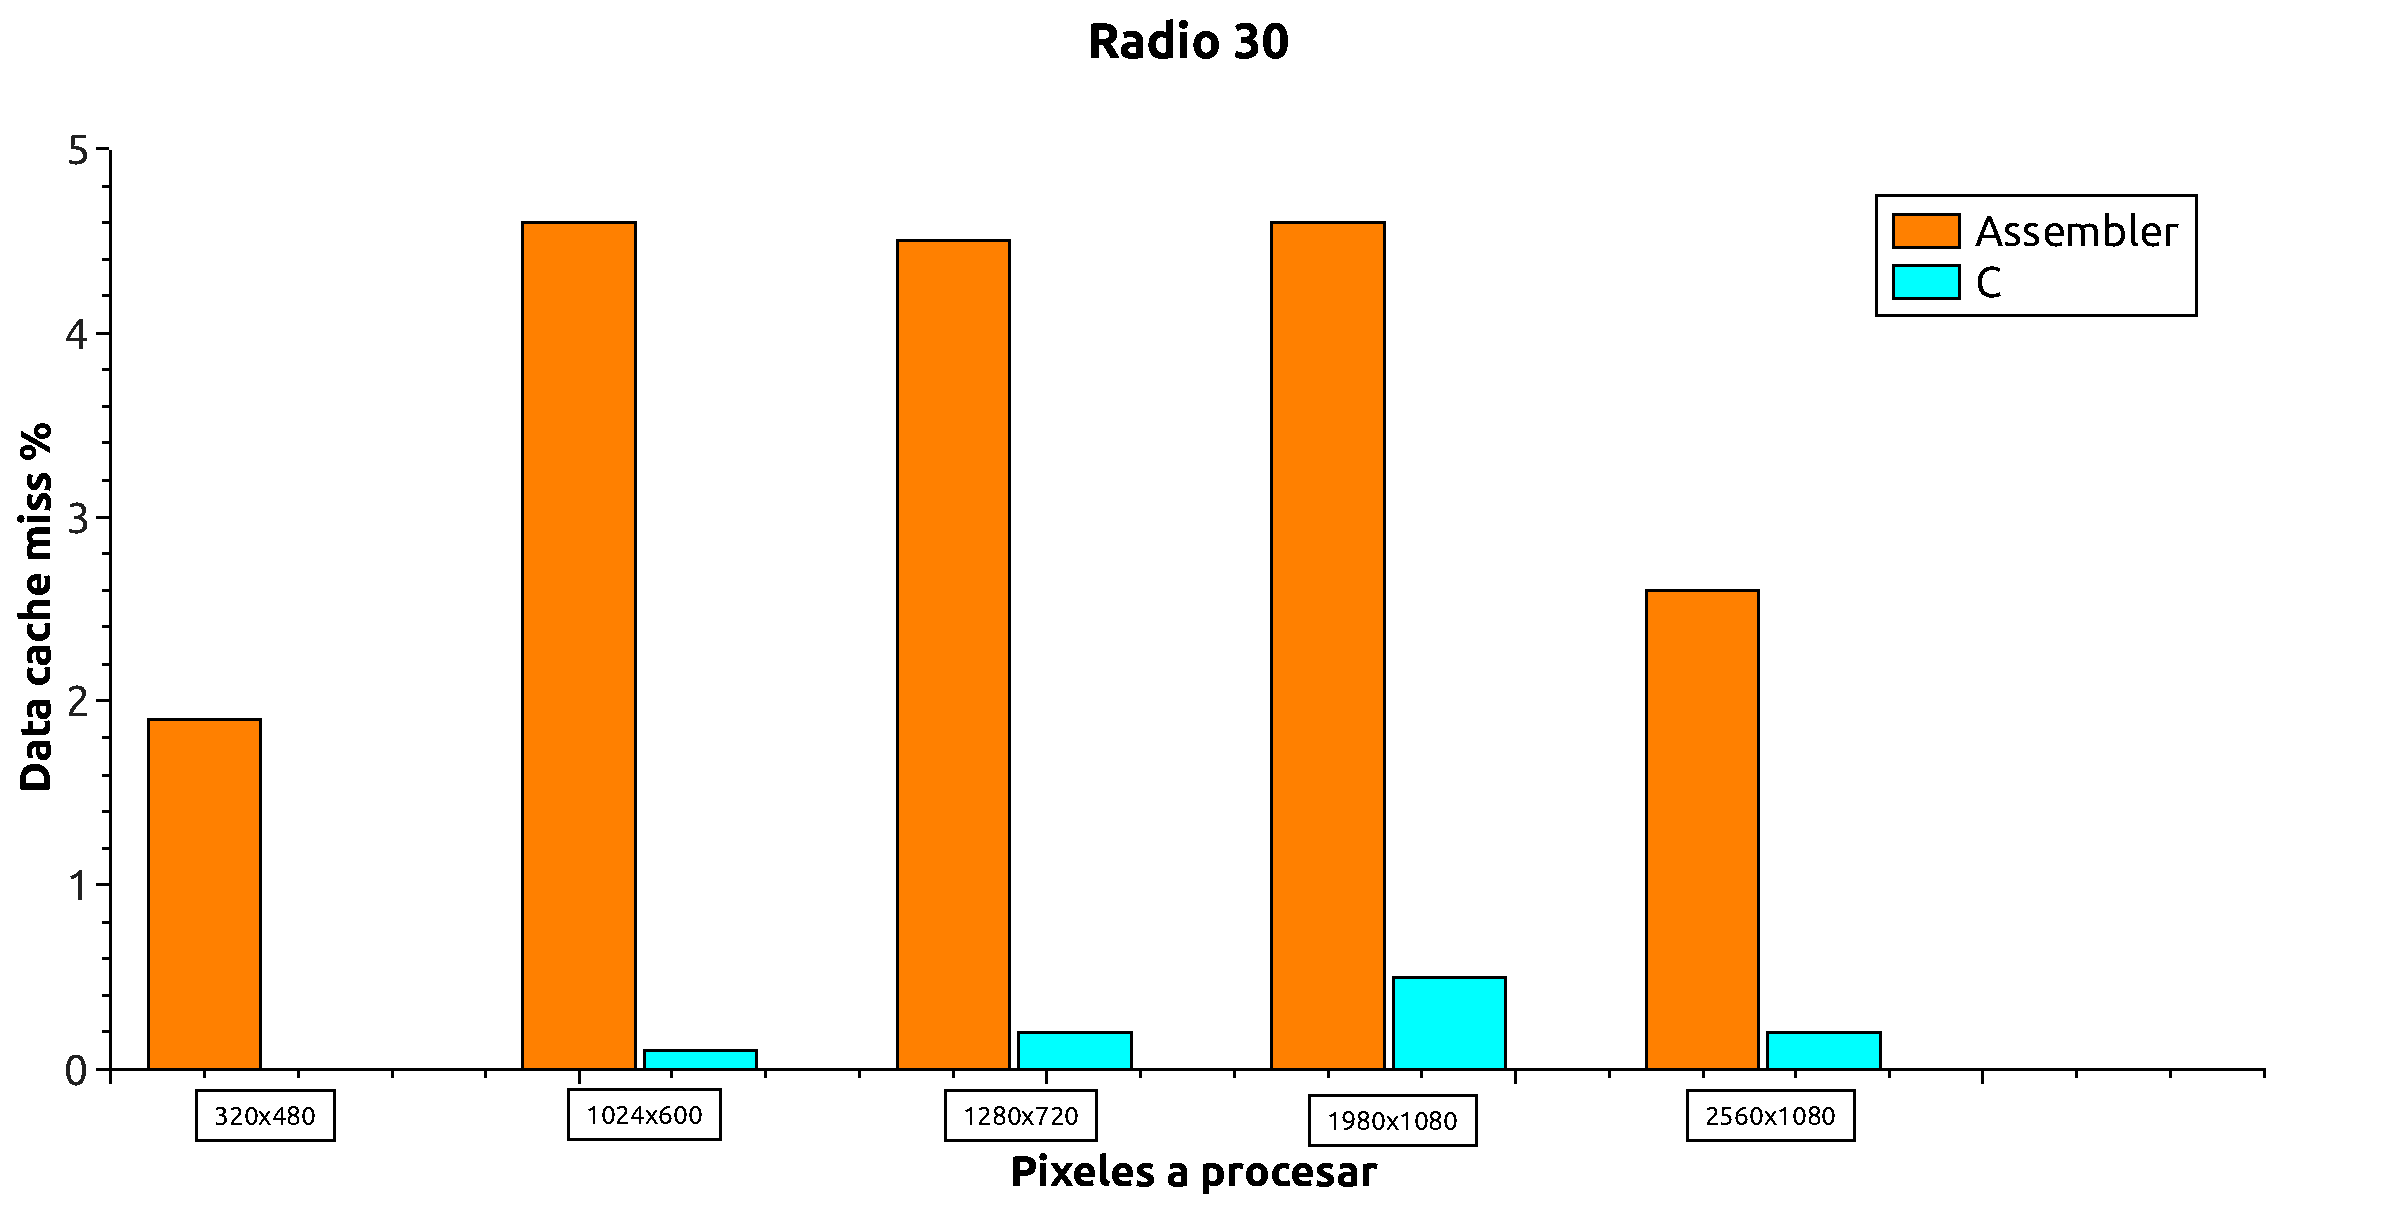
\includegraphics[width=\linewidth]{cache/Radio 30.pdf}
\end{center}
\end{figure}

\subsection{Conclusion:} \\

A partir de los graficos y de los datos obtenidos se puede ver claramente un mejor uso de la cache por parte de los filtros en c , esto va en contra de nuestra hipotesis. Sin embargo conlcuimos que esto pasa porque el compilador hace un muy buen trabajo a la hora de pasar el codigo en c a lenguaje de maquina, y que lo hace de una manera que aprovecha al maximo el uso la cache. Esta conclusion sale de que sin importar demasiado el tamaño de la imagen , el porcentaje de miss de nuestra implementacion en assembler varia muy poco a medida que aumentamos el radio y el tamaño de la imagen , mientras que la de c es siempre muy similar. Por lo tanto el tamaño de imagen y el radio no afectan el radio miss/hit de la cache. Sin embargo notamos que si bien el porcentaje de miss jumps de ambas implementaciones es muy similar, la cantidad de saltos que realiza c es muchisimo mas alta que la de asm. No inclumos estos numeros en el infome porque con un radio de 20 valgrind no terminaba de procezar la imagen , sin embargo al parar la emulacion de la cache en diferentes momentos, el porcentaje de miss era siempre el mismo, tanto en asm como en c. Con radios mas chicos la emulacion si terminaba y si se podia observar una cantidad de saltos hasta 5 veces mayor en la implementacion de c. Esto se puede atribuir a que asm utiliza simd y procesa 4 pixeles por iteracion.

